\documentclass[]{scrartcl}

\usepackage{minted}
\usepackage{mdframed}  
\usepackage{xcolor}
\usepackage{tikz}
\usepackage{tikz-3dplot}
\usetikzlibrary{matrix,decorations.pathreplacing, calc, positioning,fit}


\newcommand{\draftNote}[1]
{
	\begin{mdframed}[linewidth=0pt, backgroundcolor=red!10]
		#1
	\end{mdframed}
}


\newcommand{\draftNoteInline}[1]
{
	\textcolor{red}{(#1)}
}


%opening
\title{Documentation of swizzle and transpose functions for x86 vector registers}
\author{vhirtham}

\begin{document}		
\maketitle
\section*{About this document}
The purpose of this document is to give a short overview over the available swizzle instructions for x86 register types and the \mintinline{cpp}{Transpose} functions for matrices based on x86 vector registers.


\section{Swizzle operations}
\draftNote{
\begin{itemize}
\item Mention why template parameters -> compile time constants
\end{itemize}
}

\subsection{AlignRight}

The result of this function is equivalent to appending each lane of the second source register by each corresponding lane of the first source register and copying the 4 consecutive values starting at the index passed as template parameter to the corresponding result register lane.
The term ''right'' in the function name is adapted from the underlying intrinsic function and refers to a horizontal register representation where indices are increasing in the right-hand side direction.

\vspace{1cm}
\begin{minipage}{\linewidth}
	\subsubsection*{Example 1:}
	\begin{minted}{cpp}
	__m256 c = AlignRight<1>(a, b)
	\end{minted}
	
	\begin{tikzpicture}[>=stealth,thick,baseline, every node/.style={text height=2ex,text width=1em}]
	\plotSwizzleThreeRegisters{\colorB{1}}{\colorB{2}}{\colorB{3}}{\colorA{0}}{\colorB{5}}{\colorB{6}}{\colorB{7}}{\colorA{4}}
	
	\draw[->,color=black ]([xshift=-12pt]B-2-1.west)-- ([xshift=12pt]C-1-1.east);
	\draw[->,color=black]([xshift=-12pt]B-3-1.west)-- ([xshift= 12pt]C-2-1.east);
	\draw[->,color=black]([xshift=-12pt]B-4-1.west)-- ([xshift= 12pt]C-3-1.east);
	\draw[->,color=black ]([xshift= 12pt]A-1-1.east)-- ([xshift=-12pt]C-4-1.west);
	\draw[->,color=black ]([xshift=-12pt]B-7-1.west)-- ([xshift=12pt]C-6-1.east);
    \draw[->,color=black]([xshift=-12pt]B-8-1.west)-- ([xshift= 12pt]C-7-1.east);
    \draw[->,color=black]([xshift=-12pt]B-9-1.west)-- ([xshift= 12pt]C-8-1.east);
    \draw[->,color=black ]([xshift= 12pt]A-6-1.east)-- ([xshift=-12pt]C-9-1.west);
	\end{tikzpicture}
\end{minipage}


\vspace{1cm}
\begin{minipage}{\linewidth}
	\subsubsection*{Example 2:}
	\begin{minted}{cpp}
	__m256 c = AlignRight<2>(a, b)
	\end{minted}
	
	\begin{tikzpicture}[>=stealth,thick,baseline, every node/.style={text height=2ex,text width=1em}]
	\plotSwizzleThreeRegisters{\colorB{2}}{\colorB{3}}{\colorA{0}}{\colorA{1}}{\colorB{6}}{\colorB{7}}{\colorA{4}}{\colorA{5}}
	
	\draw[->,color=black]([xshift=-12pt]B-3-1.west)-- ([xshift= 12pt]C-1-1.east);
	\draw[->,color=black]([xshift=-12pt]B-4-1.west)-- ([xshift= 12pt]C-2-1.east);
	\draw[->,color=black ]([xshift= 12pt]A-1-1.east)-- ([xshift=-12pt]C-3-1.west);
	\draw[->,color=black ]([xshift= 12pt]A-2-1.east)-- ([xshift=-12pt]C-4-1.west);
	\draw[->,color=black]([xshift=-12pt]B-8-1.west)-- ([xshift= 12pt]C-6-1.east);
	\draw[->,color=black]([xshift=-12pt]B-9-1.west)-- ([xshift= 12pt]C-7-1.east);
	\draw[->,color=black ]([xshift= 12pt]A-6-1.east)-- ([xshift=-12pt]C-8-1.west);
	\draw[->,color=black ]([xshift= 12pt]A-7-1.east)-- ([xshift=-12pt]C-9-1.west);
	\end{tikzpicture}
\end{minipage}
\subsection{Blending}

A blend operation conditionally copies the data elements from either the first or second input registers to the same position inside a result register. 
The underlying x86 intrinsic function are \cppInline{_mm_blend_ps}, \cppInline{_mm_blend_pd}, \cppInline{_mm256_blend_ps} and \cppInline{_mm256_blend_pd}.
These functions need an integer as parameter that controls the value selection.
Several functions that calculate the control integer value based on chosen template parameters are implemented.
So it is not necessary to determine the correct integer value yourself.

On current x86 CPU architectures, blending is the most efficient swizzle operation, since multiple blends can be performed during a single CPU cycle.

\subsubsection{Blend}

The \cppInline{Blend} function has as many template parameters as data elements.
Each value van either be 0 or 1.
If a template parameter is set to 0, the corresponding data element receives its value from the first source register.
If it is 1, the value is taken from the second input register.

\subsubsection*{Example:}
\begin{minted}{cpp}
__m256 c = Blend<0, 1, 1, 0, 1, 0, 0, 0>(a, b)
\end{minted}

\begin{tikzpicture}[>=stealth,thick,baseline, every node/.style={text height=2ex,text width=1em}]
\plotSwizzleThreeRegisters{\colorA{0}}{\colorB{1}}{\colorB{2}}{\colorA{3}}{\colorB{4}}{\colorA{5}}{\colorA{6}}{\colorA{7}}

\draw[->,color=black ]([xshift= 12pt]A-1-1.east)-- ([xshift=-12pt]C-1-1.west);
\draw[->,color=black]([xshift=-12pt]B-2-1.west)-- ([xshift= 12pt]C-2-1.east);
\draw[->,color=black]([xshift=-12pt]B-3-1.west)-- ([xshift= 12pt]C-3-1.east);
\draw[->,color=black ]([xshift= 12pt]A-4-1.east)-- ([xshift=-12pt]C-4-1.west);
\draw[->,color=black]([xshift=-12pt]B-6-1.west)-- ([xshift= 12pt]C-6-1.east);
\draw[->,color=black ]([xshift= 12pt]A-7-1.east)-- ([xshift=-12pt]C-7-1.west);
\draw[->,color=black ]([xshift= 12pt]A-8-1.east)-- ([xshift=-12pt]C-8-1.west);
\draw[->,color=black ]([xshift= 12pt]A-9-1.east)-- ([xshift=-12pt]C-9-1.west);
\end{tikzpicture}


\subsubsection{BlendIndex}

The \cppInline{BlendIndex} function has only a single template parameter independent of the used register types' size.
It specifies the index of a single data element that is taken from the second source register. 
All other values are taken from the first one.

\subsubsection*{Example:}
\begin{minted}{cpp}
__m256 c = BlendIndex<5>(a, b)
\end{minted}


\begin{tikzpicture}[>=stealth,thick,baseline, every node/.style={text height=2ex,text width=1em}]
\plotSwizzleThreeRegisters{\colorA{0}}{\colorA{1}}{\colorA{2}}{\colorA{3}}{\colorA{4}}{\colorB{5}}{\colorA{6}}{\colorA{7}}

\draw[->,color=black ]([xshift= 12pt]A-1-1.east)-- ([xshift=-12pt]C-1-1.west);
\draw[->,color=black ]([xshift= 12pt]A-2-1.east)-- ([xshift=-12pt]C-2-1.west);
\draw[->,color=black ]([xshift= 12pt]A-3-1.east)-- ([xshift=-12pt]C-3-1.west);
\draw[->,color=black ]([xshift= 12pt]A-4-1.east)-- ([xshift=-12pt]C-4-1.west);
\draw[->,color=black ]([xshift= 12pt]A-6-1.east)-- ([xshift=-12pt]C-6-1.west);
\draw[->,color=black]([xshift=-12pt]B-7-1.west)-- ([xshift= 12pt]C-7-1.east);
\draw[->,color=black ]([xshift= 12pt]A-8-1.east)-- ([xshift=-12pt]C-8-1.west);
\draw[->,color=black ]([xshift= 12pt]A-9-1.east)-- ([xshift=-12pt]C-9-1.west);
\end{tikzpicture}


\subsubsection{BlendAboveIndex}

The \cppInline{BlendIndex} function has only a single template parameter independent of the used register types' size.
Data elements with a higher index than the specified value are taken from the second source register. 
All other values are taken from the first one.

\subsubsection*{Example:}
\begin{minted}{cpp}
__m256 c = BlendAboveIndex<5>(a, b)
\end{minted}

\begin{tikzpicture}[>=stealth,thick,baseline, every node/.style={text height=2ex,text width=1em}]
\plotSwizzleThreeRegisters{\colorA{0}}{\colorA{1}}{\colorA{2}}{\colorA{3}}{\colorA{4}}{\colorA{5}}{\colorB{6}}{\colorB{7}}

\draw[->,color=black ]([xshift= 12pt]A-1-1.east)-- ([xshift=-12pt]C-1-1.west);
\draw[->,color=black ]([xshift= 12pt]A-2-1.east)-- ([xshift=-12pt]C-2-1.west);
\draw[->,color=black ]([xshift= 12pt]A-3-1.east)-- ([xshift=-12pt]C-3-1.west);
\draw[->,color=black ]([xshift= 12pt]A-4-1.east)-- ([xshift=-12pt]C-4-1.west);
\draw[->,color=black ]([xshift= 12pt]A-6-1.east)-- ([xshift=-12pt]C-6-1.west);
\draw[->,color=black ]([xshift= 12pt]A-7-1.east)-- ([xshift=-12pt]C-7-1.west);
\draw[->,color=black]([xshift=-12pt]B-8-1.west)-- ([xshift= 12pt]C-8-1.east);
\draw[->,color=black]([xshift=-12pt]B-9-1.west)-- ([xshift= 12pt]C-9-1.east);
\end{tikzpicture}




\subsubsection{BlendBelowIndex}

The \cppInline{BlendIndex} function has only a single template parameter independent of the used register types' size.
Data elements with a lower index than the specified value are taken from the second source register. 
All other values are taken from the first one.

\subsubsection*{Example:}
\begin{minted}{cpp}
__m256 c = BlendBelowIndex<5>(a, b)
\end{minted}

\begin{tikzpicture}[>=stealth,thick,baseline, every node/.style={text height=2ex,text width=1em}]
\plotSwizzleThreeRegisters{\colorB{0}}{\colorB{1}}{\colorB{2}}{\colorB{3}}{\colorB{4}}{\colorA{5}}{\colorA{6}}{\colorA{7}}

\draw[->,color=black]([xshift=-12pt]B-1-1.west)-- ([xshift= 12pt]C-1-1.east);
\draw[->,color=black]([xshift=-12pt]B-2-1.west)-- ([xshift= 12pt]C-2-1.east);
\draw[->,color=black]([xshift=-12pt]B-3-1.west)-- ([xshift= 12pt]C-3-1.east);
\draw[->,color=black]([xshift=-12pt]B-4-1.west)-- ([xshift= 12pt]C-4-1.east);
\draw[->,color=black]([xshift=-12pt]B-6-1.west)-- ([xshift= 12pt]C-6-1.east);
\draw[->,color=black ]([xshift= 12pt]A-7-1.east)-- ([xshift=-12pt]C-7-1.west);
\draw[->,color=black ]([xshift= 12pt]A-8-1.east)-- ([xshift=-12pt]C-8-1.west);
\draw[->,color=black ]([xshift= 12pt]A-9-1.east)-- ([xshift=-12pt]C-9-1.west);
\end{tikzpicture}




\subsubsection{BlendInRange}

The \cppInline{BlendIndex} function has two template parameters independent of the used register types' size.
Data elements with indices equal or between those 2 values are taken from the second source register. 
All other are taken from the first one.

\subsubsection*{Example:}
\begin{minted}{cpp}
__m256 c = BlendInRange<3, 5>(a, b)
\end{minted}

\begin{tikzpicture}[>=stealth,thick,baseline, every node/.style={text height=2ex,text width=1em}]
\plotSwizzleThreeRegisters{\colorA{0}}{\colorA{1}}{\colorA{2}}{\colorB{3}}{\colorB{4}}{\colorB{5}}{\colorA{6}}{\colorA{7}}

\draw[->,color=black ]([xshift= 12pt]A-1-1.east)-- ([xshift=-12pt]C-1-1.west);
\draw[->,color=black ]([xshift= 12pt]A-2-1.east)-- ([xshift=-12pt]C-2-1.west);
\draw[->,color=black ]([xshift= 12pt]A-3-1.east)-- ([xshift=-12pt]C-3-1.west);
\draw[->,color=black]([xshift=-12pt]B-4-1.west)-- ([xshift= 12pt]C-4-1.east);
\draw[->,color=black]([xshift=-12pt]B-6-1.west)-- ([xshift= 12pt]C-6-1.east);
\draw[->,color=black]([xshift=-12pt]B-7-1.west)-- ([xshift= 12pt]C-7-1.east);
\draw[->,color=black ]([xshift= 12pt]A-8-1.east)-- ([xshift=-12pt]C-8-1.west);
\draw[->,color=black ]([xshift= 12pt]A-9-1.east)-- ([xshift=-12pt]C-9-1.west);
\end{tikzpicture}
\subsection{Broadcasting}

Broadcast operations copy a single value (per lane) from a source register to all data elements (per lane) of the result register.  

\subsubsection{Broadcast}

The \cppInline{Broadcast} function broadcast one value per lane.
The position inside the lane of the data element that should be broadcasted is passed as template parameter.
For multi-lane registers it is also possible to select different positions per lane by providing as many template parameters as the register has lanes.

\subsubsection*{Example 1:}
\begin{minted}{cpp}
__m256 b = Broadcast<2>(a)
\end{minted}

\begin{tikzpicture}[>=stealth,thick,baseline, every node/.style={text height=2ex,text width=1em}]
\plotSwizzleTwoRegisters{2}{2}{2}{2}{6}{6}{6}{6}
\draw[->,color=black ]([xshift= 12pt]A-3-1.east)-- ([xshift=-12pt]B-1-1.west);
\draw[->,color=black ]([xshift= 12pt]A-3-1.east)-- ([xshift=-12pt]B-2-1.west);
\draw[->,color=black ]([xshift= 12pt]A-3-1.east)-- ([xshift=-12pt]B-3-1.west);
\draw[->,color=black ]([xshift= 12pt]A-3-1.east)-- ([xshift=-12pt]B-4-1.west);
\draw[->,color=black ]([xshift= 12pt]A-8-1.east)-- ([xshift=-12pt]B-6-1.west);
\draw[->,color=black ]([xshift= 12pt]A-8-1.east)-- ([xshift=-12pt]B-7-1.west);
\draw[->,color=black ]([xshift= 12pt]A-8-1.east)-- ([xshift=-12pt]B-8-1.west);
\draw[->,color=black ]([xshift= 12pt]A-8-1.east)-- ([xshift=-12pt]B-9-1.west);
\end{tikzpicture}


\subsubsection*{Example 2:}
\begin{minted}{cpp}
__m256 b = Broadcast<0, 3>(a)
\end{minted}

\begin{tikzpicture}[>=stealth,thick,baseline, every node/.style={text height=2ex,text width=1em}]
\plotSwizzleTwoRegisters{0}{0}{0}{0}{7}{7}{7}{7}
\draw[->,color=black ]([xshift= 12pt]A-1-1.east)-- ([xshift=-12pt]B-1-1.west);
\draw[->,color=black ]([xshift= 12pt]A-1-1.east)-- ([xshift=-12pt]B-2-1.west);
\draw[->,color=black ]([xshift= 12pt]A-1-1.east)-- ([xshift=-12pt]B-3-1.west);
\draw[->,color=black ]([xshift= 12pt]A-1-1.east)-- ([xshift=-12pt]B-4-1.west);
\draw[->,color=black ]([xshift= 12pt]A-9-1.east)-- ([xshift=-12pt]B-6-1.west);
\draw[->,color=black ]([xshift= 12pt]A-9-1.east)-- ([xshift=-12pt]B-7-1.west);
\draw[->,color=black ]([xshift= 12pt]A-9-1.east)-- ([xshift=-12pt]B-8-1.west);
\draw[->,color=black ]([xshift= 12pt]A-9-1.east)-- ([xshift=-12pt]B-9-1.west);
\end{tikzpicture}



\subsubsection{BroadcastAcrossLanes}

For single lane registers, `BroadcastAcrossLanes` behaves the same as `Broadcast`.
For multi-lane registers, a single value selected by a template parameter is written to all data elements of the result register. 
Keep in mind, that broadcasting across lane boundaries is a rather expensive operation and should only be used if it is really necessary.

\subsubsection*{Example:}
\begin{minted}{cpp}
__m256 b = BroadcastAcrossLanes<5>(a)
\end{minted}

\begin{tikzpicture}[>=stealth,thick,baseline, every node/.style={text height=2ex,text width=1em}]
\plotSwizzleTwoRegisters{5}{5}{5}{5}{5}{5}{5}{5}
\draw[->,color=black ]([xshift= 12pt]A-7-1.east)-- ([xshift=-12pt]B-1-1.west);
\draw[->,color=black ]([xshift= 12pt]A-7-1.east)-- ([xshift=-12pt]B-2-1.west);
\draw[->,color=black ]([xshift= 12pt]A-7-1.east)-- ([xshift=-12pt]B-3-1.west);
\draw[->,color=black ]([xshift= 12pt]A-7-1.east)-- ([xshift=-12pt]B-4-1.west);
\draw[->,color=black ]([xshift= 12pt]A-7-1.east)-- ([xshift=-12pt]B-6-1.west);
\draw[->,color=black ]([xshift= 12pt]A-7-1.east)-- ([xshift=-12pt]B-7-1.west);
\draw[->,color=black ]([xshift= 12pt]A-7-1.east)-- ([xshift=-12pt]B-8-1.west);
\draw[->,color=black ]([xshift= 12pt]A-7-1.east)-- ([xshift=-12pt]B-9-1.west);
\end{tikzpicture}
\subsection{Exchange}

The \cppInline{Exchange} function modifies the passed registers directly (pass by reference) and does not return a new register.
It exchanges two values between both the registers.
The indices of the corresponding data elements are specified as template parameters.
Note that the cost of this operation is significantly higher if the exchanged values are not in the same register lane. 

\subsubsection*{Example:}
\begin{minted}{cpp}
Exchange<1, 6>(a, b)
\end{minted}

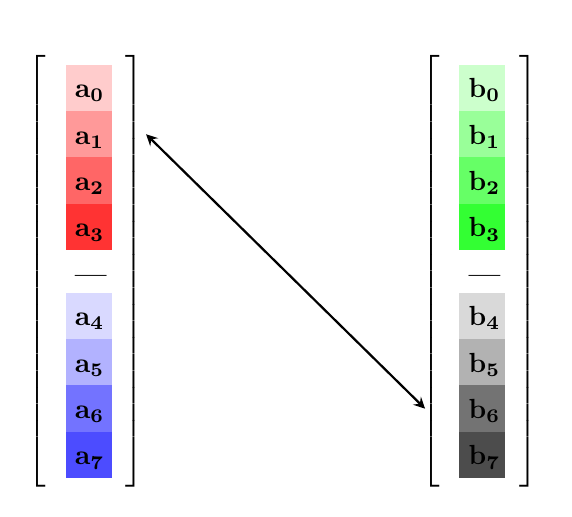
\begin{tikzpicture}[>=stealth,thick,baseline, every node/.style={text height=2ex,text width=1em}]
\matrix [matrix of math nodes,
left delimiter={[},
right delimiter={]},
](A) at (0,0){ 
	|[fill=red!20]|\mathbf{a_{0}}\\
	|[fill=red!40]|\mathbf{a_{1}}\\  
	|[fill=red!60]|\mathbf{a_{2}}\\
	|[fill=red!80]|\mathbf{a_{3}}\\
	\textbf{---}\\
	|[fill=blue!15]|\mathbf{a_{4}}\\
	|[fill=blue!30]|\mathbf{a_{5}}\\
	|[fill=blue!55]|\mathbf{a_{6}}\\
	|[fill=blue!70]|\mathbf{a_{7}}\\
};

\matrix [matrix of math nodes,
left delimiter={[},
right delimiter={]},
](B) at (5,0){ 
	|[fill=green!20]|\mathbf{b_{0}}\\
	|[fill=green!40]|\mathbf{b_{1}}\\  
	|[fill=green!60]|\mathbf{b_{2}}\\
	|[fill=green!80]|\mathbf{b_{3}}\\
	\textbf{---}\\
	|[fill=black!15]|\mathbf{b_{4}}\\
	|[fill=black!30]|\mathbf{b_{5}}\\
	|[fill=black!55]|\mathbf{b_{6}}\\
	|[fill=black!70]|\mathbf{b_{7}}\\
};

\draw[<->,color=black]([xshift= 12pt]A-2-1.east)-- ([xshift=-12pt]B-8-1.west);
\end{tikzpicture}
\hspace{1cm}
result: 
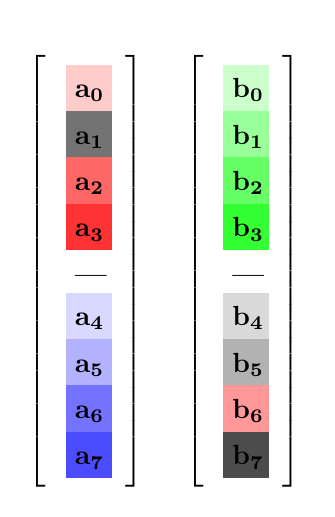
\begin{tikzpicture}[>=stealth,thick,baseline, every node/.style={text height=2ex,text width=1em}]
\matrix [matrix of math nodes,
left delimiter={[},
right delimiter={]},
](A) at (0,0){ 
	|[fill=red!20]|\mathbf{a_{0}}\\
	|[fill=black!55]|\mathbf{a_{1}}\\  
	|[fill=red!60]|\mathbf{a_{2}}\\
	|[fill=red!80]|\mathbf{a_{3}}\\
	\textbf{---}\\
	|[fill=blue!15]|\mathbf{a_{4}}\\
	|[fill=blue!30]|\mathbf{a_{5}}\\
	|[fill=blue!55]|\mathbf{a_{6}}\\
	|[fill=blue!70]|\mathbf{a_{7}}\\
};

\matrix [matrix of math nodes,
left delimiter={[},
right delimiter={]},
](B) at (2,0){ 
	|[fill=green!20]|\mathbf{b_{0}}\\
	|[fill=green!40]|\mathbf{b_{1}}\\  
	|[fill=green!60]|\mathbf{b_{2}}\\
	|[fill=green!80]|\mathbf{b_{3}}\\
	\textbf{---}\\
	|[fill=black!15]|\mathbf{b_{4}}\\
	|[fill=black!30]|\mathbf{b_{5}}\\
	|[fill=red!40]|\mathbf{b_{6}}\\
	|[fill=black!70]|\mathbf{b_{7}}\\
};
\end{tikzpicture}
\subsection{Insert}

The \cppInline{Insert} function is only defined for \cppInline{__m128} registers.
It copies a single, arbitrary value from the first passed register to an arbitrary position inside the second passed register and returns the result.
Source and destination indices are passed as template parameters.
Optionally, arbitrary values of the register can be set to 0.
This is done by 4 optional Boolean template parameters.
The Boolean values are associated with the 4 data elements of the register in ascending order.
For each one that is set to \cppInline{true}, the corresponding data element is set to 0.


\vspace{1cm}
\begin{minipage}{\linewidth}
	\subsubsection*{Example 1:}
	\begin{minted}{cpp}
__m256 c = Insert<1, 3>(a, b)
	\end{minted}
	
	\begin{tikzpicture}[>=stealth,thick,baseline, every node/.style={text height=2ex,text width=1em}]
	\plotSwizzleThreeRegistersSingleLane{\colorB{0}}{\colorB{1}}{\colorB{2}}{\colorA{1}}
	
	\draw[->,color=black ]([xshift=-12pt]B-1-1.west)-- ([xshift=12pt]C-1-1.east);
	\draw[->,color=black]([xshift=-12pt]B-2-1.west)-- ([xshift= 12pt]C-2-1.east);
	\draw[->,color=black]([xshift=-12pt]B-3-1.west)-- ([xshift= 12pt]C-3-1.east);
	\draw[->,color=black ]([xshift= 12pt]A-2-1.east)-- ([xshift=-12pt]C-4-1.west);
	\end{tikzpicture}
\end{minipage}


\vspace{1cm}
\begin{minipage}{\linewidth}
	\subsubsection*{Example 2:}
Data elements of the result register with white background have a  value of 0. 
	\begin{minted}{cpp}
__m256 c = Insert<2, 0, false, true, false, true>(a, b)
	\end{minted}
	
	\begin{tikzpicture}[>=stealth,thick,baseline, every node/.style={text height=2ex,text width=1em}]
	\plotSwizzleThreeRegistersSingleLane{\colorA{2}}{white}{\colorB{2}}{white}
	

	\draw[->,color=black]([xshift=-12pt]B-3-1.west)-- ([xshift= 12pt]C-3-1.east);
	\draw[->,color=black ]([xshift= 12pt]A-3-1.east)-- ([xshift=-12pt]C-1-1.west);
	\end{tikzpicture}
\end{minipage}
\subsection{Permute}

This function creates a new register by an arbitrary recombination of the source registers values. 
The lane value indices of the selected values are passed to the function as template parameters.

For multi-lane registers, values can not be swizzled across lane boundaries. 
Additionally, 256bit register types can either have a number of template parameters equal to the number of values per lane or equal to the number of values in the whole register.
In the first case, the permutations are identical for each lane, while in the latter case, the permutations can be chosen individually.
However, it is advised to avoid using different lane permutations for the  \cppInline{__m256} register type, since its underlying intrinsic function requires to create an additional \cppInline{__m256i} to store the indices which comes with a performance penalty.
This is not the case for the \cppInline{__m256d} register, where individual permutations have no impact on performance.

\vspace{1cm}
\begin{minipage}{\linewidth}
\subsubsection*{Example 1:}
\begin{minted}{cpp}
__m256 b = Permute<1, 3, 0, 0>(a)
\end{minted}

\begin{tikzpicture}[>=stealth,thick,baseline, every node/.style={text height=2ex,text width=1em}]
\plotSwizzleTwoRegisters{1}{3}{0}{0}{5}{7}{4}{4}
\draw[->,color=black ]([xshift= 12pt]A-2-1.east)-- ([xshift=-12pt]B-1-1.west);
\draw[->,color=black ]([xshift= 12pt]A-4-1.east)-- ([xshift=-12pt]B-2-1.west);
\draw[->,color=black ]([xshift= 12pt]A-1-1.east)-- ([xshift=-12pt]B-3-1.west);
\draw[->,color=black ]([xshift= 12pt]A-1-1.east)-- ([xshift=-12pt]B-4-1.west);
\draw[->,color=black ]([xshift= 12pt]A-7-1.east)-- ([xshift=-12pt]B-6-1.west);
\draw[->,color=black ]([xshift= 12pt]A-9-1.east)-- ([xshift=-12pt]B-7-1.west);
\draw[->,color=black ]([xshift= 12pt]A-6-1.east)-- ([xshift=-12pt]B-8-1.west);
\draw[->,color=black ]([xshift= 12pt]A-6-1.east)-- ([xshift=-12pt]B-9-1.west);
\end{tikzpicture}
\end{minipage}

\vspace{1cm}
\begin{minipage}{\linewidth}
	\subsubsection*{Example 2:}
	\begin{minted}{cpp}
__m256 b = Permute<2, 1, 3, 0, 1, 1, 3, 3>(a)
	\end{minted}
	
	\begin{tikzpicture}[>=stealth,thick,baseline, every node/.style={text height=2ex,text width=1em}]
	\plotSwizzleTwoRegisters{2}{1}{3}{0}{5}{5}{7}{7}
	\draw[->,color=black ]([xshift= 12pt]A-3-1.east)-- ([xshift=-12pt]B-1-1.west);
	\draw[->,color=black ]([xshift= 12pt]A-2-1.east)-- ([xshift=-12pt]B-2-1.west);
	\draw[->,color=black ]([xshift= 12pt]A-4-1.east)-- ([xshift=-12pt]B-3-1.west);
	\draw[->,color=black ]([xshift= 12pt]A-1-1.east)-- ([xshift=-12pt]B-4-1.west);
	\draw[->,color=black ]([xshift= 12pt]A-7-1.east)-- ([xshift=-12pt]B-6-1.west);
	\draw[->,color=black ]([xshift= 12pt]A-7-1.east)-- ([xshift=-12pt]B-7-1.west);
	\draw[->,color=black ]([xshift= 12pt]A-9-1.east)-- ([xshift=-12pt]B-8-1.west);
	\draw[->,color=black ]([xshift= 12pt]A-9-1.east)-- ([xshift=-12pt]B-9-1.west);
	\end{tikzpicture}
\end{minipage}
\subsection{Shuffle}

This function fills the lower indexed half of each result register lane with arbitrary values from the first source register.
The higher indexed half is filled with arbitrary values from the second source register.
The selected values are passed to the function as template parameters and are identical for each lane.  

\vspace{1cm}
\begin{minipage}{\linewidth}
	\subsubsection*{Example:}
	\begin{minted}{cpp}
__m256 c = Shuffle<2, 1, 3, 3>(a, b)
	\end{minted}
	
\begin{tikzpicture}[>=stealth,thick,baseline, every node/.style={text height=2ex,text width=1em}]
\plotSwizzleThreeRegisters{\colorA{2}}{\colorA{1}}{\colorB{3}}{\colorB{3}}{\colorA{6}}{\colorA{5}}{\colorB{7}}{\colorB{7}}

\draw[->,color=black ]([xshift= 12pt]A-3-1.east)-- ([xshift=-12pt]C-1-1.west);
\draw[->,color=black ]([xshift= 12pt]A-2-1.east)-- ([xshift=-12pt]C-2-1.west);
\draw[->,color=black ]([xshift=-12pt]B-4-1.west)-- ([xshift=12pt]C-3-1.east);
\draw[->,color=black]([xshift=-12pt]B-4-1.west)-- ([xshift= 12pt]C-4-1.east);
\draw[->,color=black ]([xshift= 12pt]A-8-1.east)-- ([xshift=-12pt]C-6-1.west);
\draw[->,color=black ]([xshift= 12pt]A-7-1.east)-- ([xshift=-12pt]C-7-1.west);
\draw[->,color=black ]([xshift=-12pt]B-9-1.west)-- ([xshift=12pt]C-8-1.east);
\draw[->,color=black]([xshift=-12pt]B-9-1.west)-- ([xshift= 12pt]C-9-1.east);
\end{tikzpicture}
\end{minipage}
\subsection{Swap}

This function takes a single source register, swaps 2 arbitrary values and returns the result as new register. 
The values that should be swapped are passed as template parameters.
Note that the operation is significantly more expensive if the values are swapped across lane boundaries.


\vspace{1cm}
\begin{minipage}{\linewidth}
	\subsubsection*{Example:}
	\begin{minted}{cpp}
__m256 b = Swap<1, 7>(a)
	\end{minted}
	
	\begin{tikzpicture}[>=stealth,thick,baseline, every node/.style={text height=2ex,text width=1em}]
	\plotSwizzleTwoRegisters{0}{7}{2}{3}{4}{5}{6}{1}
	\draw[->,color=black ]([xshift= 12pt]A-1-1.east)-- ([xshift=-12pt]B-1-1.west);
	\draw[->,color=black ]([xshift= 12pt]A-9-1.east)-- ([xshift=-12pt]B-2-1.west);
	\draw[->,color=black ]([xshift= 12pt]A-3-1.east)-- ([xshift=-12pt]B-3-1.west);
	\draw[->,color=black ]([xshift= 12pt]A-4-1.east)-- ([xshift=-12pt]B-4-1.west);
	\draw[->,color=black ]([xshift= 12pt]A-6-1.east)-- ([xshift=-12pt]B-6-1.west);
	\draw[->,color=black ]([xshift= 12pt]A-7-1.east)-- ([xshift=-12pt]B-7-1.west);
	\draw[->,color=black ]([xshift= 12pt]A-8-1.east)-- ([xshift=-12pt]B-8-1.west);
	\draw[->,color=black ]([xshift= 12pt]A-2-1.east)-- ([xshift=-12pt]B-9-1.west);
	\end{tikzpicture}
\end{minipage}
\subsection{Unpack functions}

The unpack functions copy values from both source registers interleaved into the result register.

\subsubsection{\_mm\_unpacklo}
This function takes from each source register lane the values that belong to the half with the low indices and copies them interleaved into the corresponding lane of the result register.

\subsubsection*{Example:}
\begin{minted}{cpp}
__m256 c = _mm_unpacklo(a, b)
\end{minted}

\begin{tikzpicture}[>=stealth,thick,baseline, every node/.style={text height=2ex,text width=1em}]
\plotSwizzleThreeRegisters{\colorA{0}}{\colorB{0}}{\colorA{1}}{\colorB{1}}{\colorA{4}}{\colorB{4}}{\colorA{5}}{\colorB{5}}

\draw[->,color=black ]([xshift= 12pt]A-1-1.east)-- ([xshift=-12pt]C-1-1.west);
\draw[->,color=black ]([xshift= 12pt]A-2-1.east)-- ([xshift=-12pt]C-3-1.west);
\draw[->,color=black ]([xshift=-12pt]B-1-1.west)-- ([xshift=12pt]C-2-1.east);
\draw[->,color=black]([xshift=-12pt]B-2-1.west)-- ([xshift= 12pt]C-4-1.east);
\draw[->,color=black ]([xshift= 12pt]A-6-1.east)-- ([xshift=-12pt]C-6-1.west);
\draw[->,color=black ]([xshift= 12pt]A-7-1.east)-- ([xshift=-12pt]C-8-1.west);
\draw[->,color=black ]([xshift=-12pt]B-6-1.west)-- ([xshift=12pt]C-7-1.east);
\draw[->,color=black]([xshift=-12pt]B-7-1.west)-- ([xshift= 12pt]C-9-1.east);
\end{tikzpicture}


\subsubsection{\_mm\_unpackhi}
This function takes from each source register lane the values that belong to the half with the high indices and copies them interleaved into the corresponding lane of the result register.

\subsubsection*{Example:}
\begin{minted}{cpp}
__m256 c = _mm_unpackhi(a, b)
\end{minted}

\begin{tikzpicture}[>=stealth,thick,baseline, every node/.style={text height=2ex,text width=1em}]
\plotSwizzleThreeRegisters{\colorA{2}}{\colorB{2}}{\colorA{3}}{\colorB{3}}{\colorA{6}}{\colorB{6}}{\colorA{7}}{\colorB{7}}

\draw[->,color=black ]([xshift= 12pt]A-3-1.east)-- ([xshift=-12pt]C-1-1.west);
\draw[->,color=black ]([xshift= 12pt]A-4-1.east)-- ([xshift=-12pt]C-3-1.west);
\draw[->,color=black ]([xshift=-12pt]B-3-1.west)-- ([xshift=12pt]C-2-1.east);
\draw[->,color=black]([xshift=-12pt]B-4-1.west)-- ([xshift= 12pt]C-4-1.east);
\draw[->,color=black ]([xshift= 12pt]A-8-1.east)-- ([xshift=-12pt]C-6-1.west);
\draw[->,color=black ]([xshift= 12pt]A-9-1.east)-- ([xshift=-12pt]C-8-1.west);
\draw[->,color=black ]([xshift=-12pt]B-8-1.west)-- ([xshift=12pt]C-7-1.east);
\draw[->,color=black]([xshift=-12pt]B-9-1.west)-- ([xshift= 12pt]C-9-1.east);
\end{tikzpicture}
\subsection{Lane Permutations}

Except for \cppInline{BroadcastAcrossLanes}, \cppInline{Exchange} and \cppInline{Swap}  all functions discussed so far did not support swizzling across lane boundaries.
The functions of this section provide a way to permute register lanes.
They are also used internally by \cppInline{BroadcastAcrossLanes}, \cppInline{Exchange} and \cppInline{Swap} to transfer values between different lanes.
The high latency of lane permutations (see intel intrinsics guide) are responsible for the increased computational effort of those 3 functions and why they should be used with care.

\subsubsection{Permute2F128} 

This function has 2 overloads and creates a new register by recombining the lanes of 1 or 2 source registers.
It can only be used with 256 bit registers.

The first overload is called with 2 source registers and requires 4 template parameters.
The first and second template parameter determine the source register and which of its lanes should be copied to the first lane of the result register.
The remaining 2 template parameters specify source register and lane for the second lane of the result register.

The second overload takes a single source register and 2 template parameters that define which lanes of the source register are copied to the first and second lane of the result register.   

 \vspace{1cm}
 \begin{minipage}{\linewidth}
 	\subsubsection*{Example 1:}
 	\begin{minted}{cpp}
__m256 c = Permute2F128<0, 1, 1, 1>(a, b)
 	\end{minted}
 	
 	\begin{tikzpicture}[>=stealth,thick,baseline, every node/.style={text height=2ex,text width=1em}]
 	\plotSwizzleThreeRegisters{\colorA{4}}{\colorA{5}}{\colorA{6}}{\colorA{7}}{\colorB{4}}{\colorB{5}}{\colorB{6}}{\colorB{7}}
 	
 	\draw[->,color=black]([xshift= 12pt]A-6-1.east)-- ([xshift= -12pt]C-1-1.west);
 	\draw[->,color=black]([xshift= 12pt]A-7-1.east)-- ([xshift= -12pt]C-2-1.west);
 	\draw[->,color=black ]([xshift= 12pt]A-8-1.east)-- ([xshift=-12pt]C-3-1.west);
 	\draw[->,color=black ]([xshift= 12pt]A-9-1.east)-- ([xshift=-12pt]C-4-1.west);
 	\draw[->,color=black]([xshift=-12pt]B-6-1.west)-- ([xshift= 12pt]C-6-1.east);
 	\draw[->,color=black]([xshift=-12pt]B-7-1.west)-- ([xshift= 12pt]C-7-1.east);
 	\draw[->,color=black ]([xshift= -12pt]B-8-1.west)-- ([xshift= 12pt]C-8-1.east);
 	\draw[->,color=black ]([xshift= -12pt]B-9-1.west)-- ([xshift= 12pt]C-9-1.east);
 	\end{tikzpicture}
 \end{minipage}

\vspace{1cm}
\begin{minipage}{\linewidth}
	\subsubsection*{Example 2:}
	\begin{minted}{cpp}
__m256 b = Permute2F128<0, 0>(a)
	\end{minted}
	
	\begin{tikzpicture}[>=stealth,thick,baseline, every node/.style={text height=2ex,text width=1em}]
	\plotSwizzleTwoRegisters{0}{1}{2}{3}{0}{1}{2}{3}
	\draw[->,color=black ]([xshift= 12pt]A-1-1.east)-- ([xshift=-12pt]B-1-1.west);
	\draw[->,color=black ]([xshift= 12pt]A-2-1.east)-- ([xshift=-12pt]B-2-1.west);
	\draw[->,color=black ]([xshift= 12pt]A-3-1.east)-- ([xshift=-12pt]B-3-1.west);
	\draw[->,color=black ]([xshift= 12pt]A-4-1.east)-- ([xshift=-12pt]B-4-1.west);
	\draw[->,color=black ]([xshift= 12pt]A-1-1.east)-- ([xshift=-12pt]B-6-1.west);
	\draw[->,color=black ]([xshift= 12pt]A-2-1.east)-- ([xshift=-12pt]B-7-1.west);
	\draw[->,color=black ]([xshift= 12pt]A-3-1.east)-- ([xshift=-12pt]B-8-1.west);
	\draw[->,color=black ]([xshift= 12pt]A-4-1.east)-- ([xshift=-12pt]B-9-1.west);
	\end{tikzpicture}
\end{minipage}



\subsection{Permute4F64 and Permute8F32}

These two functions can be used to create a new register with arbitrary value recombination of the source register.
Values can also be copied across lane boundaries.
\cppInline{Permute4F64} only works with \cppInline{__m256d} registers and needs 4 template parameters that specify the selected values.
\cppInline{Permute8F32} is for \cppInline{__m256} registers and needs 8 template parameters.
Note that \cppInline{Permute8F32} has extra computational costs, since it requires the creation of an additional \cppInline{__m256i} register for the indices while this is not the case for \cppInline{Permute4F64}.

 
\vspace{1cm}
\begin{minipage}{\linewidth}
	\subsubsection*{Example:}
	\begin{minted}{cpp}
__m256 b = Permute8F32<1, 5, 6, 1, 7, 0, 2, 2>(a)
	\end{minted}
	
	\begin{tikzpicture}[>=stealth,thick,baseline, every node/.style={text height=2ex,text width=1em}]
	\plotSwizzleTwoRegisters{1}{5}{6}{1}{7}{0}{2}{2}
	\draw[->,color=black ]([xshift= 12pt]A-2-1.east)-- ([xshift=-12pt]B-1-1.west);
	\draw[->,color=black ]([xshift= 12pt]A-7-1.east)-- ([xshift=-12pt]B-2-1.west);
	\draw[->,color=black ]([xshift= 12pt]A-8-1.east)-- ([xshift=-12pt]B-3-1.west);
	\draw[->,color=black ]([xshift= 12pt]A-2-1.east)-- ([xshift=-12pt]B-4-1.west);
	\draw[->,color=black ]([xshift= 12pt]A-9-1.east)-- ([xshift=-12pt]B-6-1.west);
	\draw[->,color=black ]([xshift= 12pt]A-1-1.east)-- ([xshift=-12pt]B-7-1.west);
	\draw[->,color=black ]([xshift= 12pt]A-3-1.east)-- ([xshift=-12pt]B-8-1.west);
	\draw[->,color=black ]([xshift= 12pt]A-3-1.east)-- ([xshift=-12pt]B-9-1.west);
	\end{tikzpicture}
\end{minipage}



\subsubsection{SwapLanes and SwapLanesIf}

The \cppInline{SwapLanes} function takes a single 256 bit register and returns a new one with swapped lanes.

\cppInline{SwapLanesIF} is a conditional version of the \cppInline{SwapLanes} function.
If the required template parameter is \cppInline{true} the function calls \cppInline{SwapLanes} and returns the result.
If it is \cppInline{false}, a copy of the unmodified source register is returned.



\vspace{1cm}
\begin{minipage}{\linewidth}
	\subsubsection*{Example 1:}
	\begin{minted}{cpp}
__m256 b = SwapLanes(a)
	\end{minted}
	and
	\begin{minted}{cpp}
__m256 b = SwapLanesIf<true>(a)
	\end{minted}
	\begin{tikzpicture}[>=stealth,thick,baseline, every node/.style={text height=2ex,text width=1em}]
	\plotSwizzleTwoRegisters{4}{5}{6}{7}{0}{1}{2}{3}
	\draw[->,color=black ]([xshift= 12pt]A-6-1.east)-- ([xshift=-12pt]B-1-1.west);
	\draw[->,color=black ]([xshift= 12pt]A-7-1.east)-- ([xshift=-12pt]B-2-1.west);
	\draw[->,color=black ]([xshift= 12pt]A-8-1.east)-- ([xshift=-12pt]B-3-1.west);
	\draw[->,color=black ]([xshift= 12pt]A-9-1.east)-- ([xshift=-12pt]B-4-1.west);
	\draw[->,color=black ]([xshift= 12pt]A-1-1.east)-- ([xshift=-12pt]B-6-1.west);
	\draw[->,color=black ]([xshift= 12pt]A-2-1.east)-- ([xshift=-12pt]B-7-1.west);
	\draw[->,color=black ]([xshift= 12pt]A-3-1.east)-- ([xshift=-12pt]B-8-1.west);
	\draw[->,color=black ]([xshift= 12pt]A-4-1.east)-- ([xshift=-12pt]B-9-1.west);
	\end{tikzpicture}
\end{minipage}


\vspace{1cm}
\begin{minipage}{\linewidth}
	\subsubsection*{Example 2:}
	\begin{minted}{cpp}
__m256 b = SwapLanesIf<false>(a)
	\end{minted}
	
	\begin{tikzpicture}[>=stealth,thick,baseline, every node/.style={text height=2ex,text width=1em}]
	\plotSwizzleTwoRegisters{0}{1}{2}{3}{4}{5}{6}{7}
	\draw[->,color=black ]([xshift= 12pt]A-1-1.east)-- ([xshift=-12pt]B-1-1.west);
	\draw[->,color=black ]([xshift= 12pt]A-2-1.east)-- ([xshift=-12pt]B-2-1.west);
	\draw[->,color=black ]([xshift= 12pt]A-3-1.east)-- ([xshift=-12pt]B-3-1.west);
	\draw[->,color=black ]([xshift= 12pt]A-4-1.east)-- ([xshift=-12pt]B-4-1.west);
	\draw[->,color=black ]([xshift= 12pt]A-6-1.east)-- ([xshift=-12pt]B-6-1.west);
	\draw[->,color=black ]([xshift= 12pt]A-7-1.east)-- ([xshift=-12pt]B-7-1.west);
	\draw[->,color=black ]([xshift= 12pt]A-8-1.east)-- ([xshift=-12pt]B-8-1.west);
	\draw[->,color=black ]([xshift= 12pt]A-9-1.east)-- ([xshift=-12pt]B-9-1.west);
	\end{tikzpicture}
\end{minipage}










\section{Transpose functions}

\subsection{Introduction}
Transposing a matrix that uses an array of fundamental scalar types (\cppInline{int}, \cppInline{float}, \cppInline{double}, etc.) as underlying data structure is rather easy to implement.
For an arbitrary $M \times N$ matrix the implementation could look like the following piece of code:

\begin{minted}{cpp}
for (U32 i = 0; i < N; ++i)
    for (U32 j = 0; j < M; ++j)
        transposed[j + i * cols] = original[i + j * rows];
\end{minted}

If an array of vector register types (\cppInline{__m128},\cppInline{__m128d}, \cppInline{__m256}, etc.) is utilized to store the matrix's data, it gets more complicated.
This section describes the special transpose functions for x86 registers and how they can be used.
Additionally, some details of the implementation are discussed.

\subsection{Matrix format}
\label{sec:transpose_matrix_format}
In this section, we consider only matrices that are stored in column-major format and with a maximum size of $\numRegisterElements \times \numRegisterElements$, where $\numRegisterElements$ is the number of elements of the underlying register type.
By using $\numRegisterElements \times \numRegisterElements$ matrices as basic building blocks, any larger $M \times N$ matrix can be transposed by using the following rule:

\begin{align}
\label{eq:block_matrix_transpose}
M =
\begin{bmatrix}
A_{11} & A_{12} & \cdots & A_{1j}\\
A_{21} & A_{22} & \cdots & A_{2j}\\
\vdots & \vdots & \ddots &\vdots \\
A_{i1} & A_{i2} & \cdots & A_{ij}\\
\end{bmatrix} && 
M^T =
\begin{bmatrix}
A_{11}^T & A_{21}^T & \cdots & A_{i1}^T\\
A_{12}^T & A_{22}^T & \cdots & A_{i2}^T\\
\vdots   & \vdots   & \ddots &\vdots \\
A_{1j}^T & A_{2j}^T & \cdots & A_{ij}^T\\
\end{bmatrix}  
\end{align}

\noindent Here all $A$ are $\numRegisterElements \times \numRegisterElements$ sub-matrices.


Each column of a matrix is stored in its own register.
This does not change, even if that means that some memory is wasted in case a matrix has less than $\numRegisterElements$ rows.
So an $2 \times 2$ matrix that is stored in an array of \cppInline{__m128} registers (4 elements per register) will still use 2 registers (one for each column), even though the data fits into a single one.

Additionally, the first row of a matrix with less than $\numRegisterElements$ rows mustn't necessarily be stored inside the first elements of the column registers. 
The only condition is that each column of the matrix is stored contiguously in ascending order and the offset is identical in each register of the matrix.
While one should usually avoid storing individual matrices with offsets, this gets important if only a sub-matrix of a $\numRegisterElements \times \numRegisterElements$ matrix should be transposed.
 

\subsection{Available functions}

\subsubsection{Size specific functions}

Each register type has its own set of transpose functions available in a corresponding header.
For example, for \cppInline{__m128} registers, you have to use
\begin{minted}{cpp}
#include "gdl/base/simd/_transpose/transpose_m128.h"
\end{minted}

The headers contain one function for each matrix size up to $\numRegisterElements \times \numRegisterElements$.
They are named ''Transpose'' plus the matrix size.
So for a $2 \times 4$ matrix, the function \cppInline{Transpose2x4} has to be used.

The functions only take registers of the utilized type as parameters.
Their number depends on the matrix size and is equal to the number of columns plus the number of rows.
The first $N$ parameters are the columns register of the $M \times N$ source matrix in ascending order.
The last $M$ parameters are references to the columns register of the $N \times M$ target matrix in ascending order.
Results of the transposition will be written directly to the passed registers of the target matrix.
Therefore, the functions do not return anything.

Furthermore, each function takes 4 optional template parameters.
The first parameter must be an integer that specifies the offset of the source matrix's first row inside its column registers (see \cref{sec:transpose_matrix_format}).
Default value is 0.
The second template parameter is also an integer and specifies the register offset of the target matrix's first row (default is 0).
Using these 2 parameters lets you read a sub-matrix at an arbitrary position of the source matrix and write the transposed result to an arbitrary location of a target matrix.

The third template parameter is a \cppInline{bool}.
Setting it to \cppInline{false} prevents the function from modifying any memory of the target matrix registers that is not needed to store the result of the transposition.
However, it is faster to use \cppInline{true} (default) since the limited set of swizzle operations requires additional blending instructions to keep values that shouldn't be modified in place.
In this case, the memory outside the result matrix's memory range usually contains meaningless garbage.
Make sure to only select \cppInline{false} as third template parameter if it is really necessary to get the best performance.

The fourth and last parameter is also a \cppInline{bool}.
It has only a meaning if the third parameter is set to \cppInline{true}.
By setting it to \cppInline{true}, all unused memory of the result registers is overwritten with 0.
In most cases, this requires additional instruction. 
Only the \cppInline{__m128} register has some functions where this is not the case due to the utilization of the \cppInline{Insert} function.
So this should always be set to \cppInline{false} (default) if it is not needed.

\subsubsection*{Examples}

The following examples show the Transposition of $3 \times 2$ matrix $\textrm{A}$ using different template parameter combinations. 
Its underlying data is the \cppInline{std::array<__m256, 2> a}.
The $2 \times 3$ result matrix $\textrm{B}$ has the \cppInline{std::array<__m256, 3> b} as underlying data structure.
Each register of the arrays contains a single matrix column as defined in \cref{sec:transpose_matrix_format}.

Since a single \cppInline{__m256} register contains 8 values, the matrix $\textrm{A}$ is actually visualized as an $8 \times 2$ matrix.
The relevant $3 \times 2$ block is marked in blue.

Similarly, the matrix $\textrm{B}$ is visualized twice as a $8 \times 3$ matrix.
Once before and once after the transposition.
The target area that receives the result values is marked green.
In case that values of $\textrm{B}$ are overwritten, even though they are not part of the result matrix, they are marked in red.
An ''$\times$'' in $\textrm{B}$ after the transposition means that the corresponding value is undefined/random.


\vspace{1cm}
\begin{minipage}{\linewidth}
\begin{minted}{cpp}
Transpose3x2(a[0], a[1], b[0], b[1], b[2]);
\end{minted}
equivalent to: 
\begin{minted}{cpp}
Transpose3x2<0 ,0 , true, false>(a[0], a[1], b[0], b[1], b[2]);
\end{minted}
yields:

\begin{align*}
\begin{matrix}
\textrm{Matrix A} & \textrm{Matrix B}  & & \textrm{Matrix B}\\
&\textrm{(before transposition)}&&\textrm{(after transposition)}\\
\\
\left(\begin{array}{cc}
\colSrc 0 & \colSrc 8\\
\colSrc 1 & \colSrc 9\\
\colSrc 2 & \colSrc 10\\
3 & 11\\
4 & 12\\
5 & 13\\
6 & 14\\
7 & 15
\end{array}\right) 
&
\left(\begin{array}{ccc}
\colTgt 100 & \colTgt 108 & \colTgt 116\\
\colTgt 101 & \colTgt 109 & \colTgt 117\\
\colOwr 102 & \colOwr 110 & \colOwr 118\\
\colOwr 103 & \colOwr 111 & \colOwr 119\\
\colOwr 104 & \colOwr 112 & \colOwr 120\\
\colOwr 105 & \colOwr 113 & \colOwr 121\\
\colOwr 106 & \colOwr 114 & \colOwr 122\\
\colOwr 107 & \colOwr 115 & \colOwr 123
\end{array}\right) 
&&
\left(\begin{array}{ccc}
0      & 1      & 2\\
8      & 9      & 10\\
\times & \times & \times\\
\times & \times & \times\\
\times & \times & \times\\
\times & \times & \times\\
\times & \times & \times\\
\times & \times & \times\\
\end{array}\right) 
\end{matrix}
\end{align*}
\end{minipage}


\vspace{2cm}
\begin{minipage}{\linewidth}
	\begin{minted}{cpp}
Transpose3x2<4 ,2 , true, true>(a[0], a[1], b[0], b[1], b[2]);
	\end{minted}
	yields:
	\begin{align*}
	\begin{matrix}
	\textrm{Matrix A} & \textrm{Matrix B}  & & \textrm{Matrix B}\\
	&\textrm{(before transposition)}&&\textrm{(after transposition)}\\
	\\
	\left(\begin{array}{cc}
	0 & 8\\
	1 & 9\\
	2 & 10\\
	3 & 11\\
	\colSrc 4 & \colSrc 12\\
	\colSrc 5 & \colSrc 13\\
	\colSrc 6 & \colSrc 14\\
	7 & 15
	\end{array}\right) 
	&
	\left(\begin{array}{ccc}
	\colOwr 100 & \colOwr 108 & \colOwr 116\\
	\colOwr 101 & \colOwr 109 & \colOwr 117\\
	\colTgt 102 & \colTgt 110 & \colTgt 118\\
	\colTgt 103 & \colTgt 111 & \colTgt 119\\
	\colOwr 104 & \colOwr 112 & \colOwr 120\\
	\colOwr 105 & \colOwr 113 & \colOwr 121\\
	\colOwr 106 & \colOwr 114 & \colOwr 122\\
	\colOwr 107 & \colOwr 115 & \colOwr 123
	\end{array}\right) 
	&&
	\left(\begin{array}{ccc}
	0 & 0 & 0\\
	0 & 0 & 0\\
	4 & 5 & 6\\
	12 & 13 & 14\\
	0 & 0 & 0\\
	0 & 0 & 0\\
	0 & 0 & 0\\
	0 & 0 & 0	
	\end{array}\right) 
	\end{matrix}
	\end{align*}
\end{minipage}

\vspace{2cm}
\begin{minipage}{\linewidth}
	\begin{minted}{cpp}
Transpose3x2<1 ,6 , false, false>(a[0], a[1], b[0], b[1], b[2]);
	\end{minted}
	yields:
	\begin{align*}
	\begin{matrix}
	\textrm{Matrix A} & \textrm{Matrix B}  & & \textrm{Matrix B}\\
	&\textrm{(before transposition)}&&\textrm{(after transposition)}\\
	\\
	\left(\begin{array}{cc}
	0 & 8\\
	\colSrc 1 & \colSrc 9\\
	\colSrc 2 & \colSrc 10\\
	\colSrc 3 & \colSrc 11\\
	4 & 12\\
    5 & 13\\
	6 & 14\\
	7 & 15
	\end{array}\right) 
	&
	\left(\begin{array}{ccc}
	100 & 108 & 116\\
	101 & 109 & 117\\
	102 & 110 & 118\\
	103 & 111 & 119\\
	104 & 112 & 120\\
	105 & 113 & 121\\
	\colTgt 106 & \colTgt 114 & \colTgt 122\\
	\colTgt 107 & \colTgt 115 & \colTgt 123
	\end{array}\right) 
	&&
	\left(\begin{array}{ccc}
    100 & 108 & 116\\
    101 & 109 & 117\\
    102 & 110 & 118\\
    103 & 111 & 119\\
    104 & 112 & 120\\
    105 & 113 & 121\\
    1 & 2 & 3\\
    9 & 10 & 11
\end{array}\right) 
	\end{matrix}
	\end{align*}
\end{minipage}

\subsubsection{General purpose function}

Having a separate transpose function for each matrix size limits flexibility.
The general purpose function wraps all size and register specific transpose functions into a large compile time switch that can be controlled by the functions template parameters.
It can be included with:

\begin{minted}{cpp}
#include "gdl/base/simd/transpose.h"
\end{minted}

Instead of passing each of the matrices' underlying registers separately, the source matrix data and the target matrix data are both passed as a \cppInline{std::array} of the corresponding register type.
The minimal size of the array must fulfill the storage requirements of the matrix format defined in \cref{sec:transpose_matrix_format}, but it might also be larger.
Special offset and stride template parameters can be used to select the registers that belong to the source and target matrix inside arbitrary over-sized arrays.
This functionality can be used to transpose matrices of any size that are stored inside a continuous register array by using \cref{eq:block_matrix_transpose}.

The function has 10 template parameter options to modify its behavior.
The matrix size is selected with the first 2 parameters, with the number of rows being the first parameter.
If the selected size exceeds the register specific limitations, a corresponding static assertion will fail.
Parameter 3 and 4 define the offsets of the source and target matrix's first row inside their corresponding registers (see \cref{sec:transpose_matrix_format}).
They are internally past as the first two template parameters to the corresponding size specific function.
The default value is 0.
The parameters 5 and 6 specify the index of the matrices first column registers inside their corresponding data array (default 0).
Parameter 7 and 8 are the stride between to matrix registers inside the data arrays (default 1).
The last 2 parameters are Boolean switches that specify how register memory of the target matrix is handled, that is not needed to store the result.
Their order, default values and functionality are identical to the third and fourth template parameter of the size specific functions described in the previous section.


\subsubsection*{Examples}

The following examples show different applications of the general purpose \cppInline{Transpose} function.
The arrays \cppInline{std::array<__m256, 6> a} and \cppInline{std::array<__m256, 5> b} will be used as input parameters. 
They are visualized as a matrix, where each column represents a single register.
As in the previous section, the array \cppInline{b} will be shown before and after the operation.
Areas colored in blue mark the source values in the array \cppInline{a}.
Entries of the array \cppInline{b}, that will be overwritten by the result matrix, are colored green.
Red areas mark values that are not part of the result matrix but will be overwritten by the function.
An $\times$ in the representation of \cppInline{b} after the transposition represents an undefined value (random value from the source matrix).

\vspace{1cm}
\begin{minipage}{\linewidth}
	\begin{minted}{cpp}
Transpose<3, 2>(a, b);
	\end{minted}
	equivalent to: 
	\begin{minted}{cpp}
Transpose<3, 2, 0, 0, 0, 0, 1, 1, true, false>(a, b);
	\end{minted}
	yields:
	
	\begin{align*}
	\begin{matrix}
	\textrm{array a} & \textrm{array b}  & & \textrm{array b}\\
	&\textrm{(before transposition)}&&\textrm{(after transposition)}\\
	\\
	\left(\begin{array}{cccccc}
	\colSrc 0 & \colSrc 8  & 16 & 24 & 32 & 40\\
	\colSrc 1 & \colSrc 9  & 17 & 25 & 33 & 41\\
	\colSrc 2 & \colSrc 10 & 18 & 26 & 34 & 42\\
	3 & 11 & 19 & 27 & 35 & 43\\
    4 & 12 & 20 & 28 & 36 & 44\\
    5 & 13 & 21 & 29 & 37 & 45\\
    6 & 14 & 22 & 30 & 38 & 46\\
    7 & 15 & 23 & 31 & 39 & 47
	\end{array}\right) 
	&
	\left(\begin{array}{ccccc}
	\colTgt 60 & \colTgt 68 & \colTgt 76 & 84 & 92\\
	\colTgt 61 & \colTgt 69 & \colTgt 77 & 85 & 93\\
	\colOwr 62 & \colOwr 70 & \colOwr 78 & 86 & 94\\
	\colOwr 63 & \colOwr 71 & \colOwr 79 & 87 & 95\\
	\colOwr 64 & \colOwr 72 & \colOwr 80 & 88 & 96\\
	\colOwr 65 & \colOwr 73 & \colOwr 81 & 89 & 97\\
	\colOwr 66 & \colOwr 74 & \colOwr 82 & 90 & 98\\
	\colOwr 67 & \colOwr 75 & \colOwr 83 & 91 & 99
	\end{array}\right) 
	&&
	\left(\begin{array}{ccccc}
	0      & 1      & 2      & 84 & 92\\
	8      & 9      & 10     & 85 & 93\\
	\times & \times & \times & 86 & 94\\
	\times & \times & \times & 87 & 95\\
	\times & \times & \times & 88 & 96\\
	\times & \times & \times & 89 & 97\\
	\times & \times & \times & 90 & 98\\
	\times & \times & \times & 91 & 99
	\end{array}\right)
	\end{matrix}
	\end{align*}
\end{minipage}



\vspace{1cm}
\begin{minipage}{\linewidth}
	\begin{minted}{cpp}
Transpose<2, 2, 6, 3, 2, 1, 1, 1, true, true>(a, b);
	\end{minted}
	yields:
	
	\begin{align*}
	\begin{matrix}
	\textrm{array a} & \textrm{array b}  & & \textrm{array b}\\
	&\textrm{(before transposition)}&&\textrm{(after transposition)}\\
	\\
	\left(\begin{array}{cccccc}
	0 & 8  & 16         & 24         & 32 & 40\\
	1 & 9  & 17         & 25         & 33 & 41\\
	2 & 10 & 18         & 26         & 34 & 42\\
	3 & 11 & 19         & 27         & 35 & 43\\
	4 & 12 & 20         & 28         & 36 & 44\\
	5 & 13 & 21         & 29         & 37 & 45\\
	6 & 14 & \colSrc 22 & \colSrc 30 & 38 & 46\\
	7 & 15 & \colSrc 23 & \colSrc 31 & 39 & 47
	\end{array}\right) 
	&
	\left(\begin{array}{ccccc}
	60 & \colOwr 68 & \colOwr 76 & 84 & 92\\
	61 & \colOwr 69 & \colOwr 77 & 85 & 93\\
	62 & \colOwr 70 & \colOwr 78 & 86 & 94\\
	63 & \colTgt 71 & \colTgt 79 & 87 & 95\\
	64 & \colTgt 72 & \colTgt 80 & 88 & 96\\
	65 & \colOwr 73 & \colOwr 81 & 89 & 97\\
	66 & \colOwr 74 & \colOwr 82 & 90 & 98\\
	67 & \colOwr 75 & \colOwr 83 & 91 & 99
	\end{array}\right) 
	&&
	\left(\begin{array}{ccccc}
	60 & 0  & 0  & 84 & 92\\
	61 & 0  & 0  & 85 & 93\\
	62 & 0  & 0  & 86 & 94\\
	63 & 22 & 23 & 87 & 95\\
	64 & 30 & 31 & 88 & 96\\
	65 & 0  & 0  & 89 & 97\\
	66 & 0  & 0  & 90 & 98\\
	67 & 0  & 0  & 91 & 99
	\end{array}\right)
	\end{matrix}
	\end{align*}
\end{minipage}



\vspace{1cm}
\begin{minipage}{\linewidth}
	\begin{minted}{cpp}
	Transpose<2, 3, 1, 3, 0, 1, 2, 3, false, false>(a, b);
	\end{minted}
	yields:
	
	\begin{align*}
	\begin{matrix}
	\textrm{array a} & \textrm{array b}  & & \textrm{array b}\\
	&\textrm{(before transposition)}&&\textrm{(after transposition)}\\
	\\
	\left(\begin{array}{cccccc}
	0         & 8  & 16         & 24 & 32         & 40\\
	\colSrc 1 & 9  & \colSrc 17 & 25 & \colSrc 33 & 41\\
	\colSrc 2 & 10 & \colSrc 18 & 26 & \colSrc 34 & 42\\
	3         & 11 & 19         & 27 & 35         & 43\\
	4         & 12 & 20         & 28 & 36         & 44\\
	5         & 13 & 21         & 29 & 37         & 45\\
	6         & 14 & 22         & 30 & 38         & 46\\
	7         & 15 & 23         & 31 & 39         & 47
	\end{array}\right) 
	&
	\left(\begin{array}{ccccc}
	60 & 68         & 76 & 84 & 92\\
	61 & 69         & 77 & 85 & 93\\
	62 & 70         & 78 & 86 & 94\\
	63 & \colTgt 71 & 79 & 87 & \colTgt 95\\
	64 & \colTgt 72 & 80 & 88 & \colTgt 96\\
	65 & \colTgt 73 & 81 & 89 & \colTgt 97\\
	66 & 74         & 82 & 90 & 98\\
	67 & 75         & 83 & 91 & 99
	\end{array}\right) 
	&&
	\left(\begin{array}{ccccc}
	60 & 68 & 76 & 84 & 92\\
	61 & 69 & 77 & 85 & 93\\
	62 & 70 & 78 & 86 & 94\\
	63 & 1  & 79 & 87 & 2\\
	64 & 17 & 80 & 88 & 18\\
	65 & 33 & 81 & 89 & 34\\
	66 & 74 & 82 & 90 & 98\\
	67 & 75 & 83 & 91 & 99
	\end{array}\right)
	\end{matrix}
	\end{align*}
\end{minipage}



\subsection{Implementation details}
The challenge is to find the most effective combination of swizzle instructions (see previous section) to perform the transposition.
Unfortunately, the optimal combination depends on the matrix size.




\end{document}